\section{Motivation}

In this chapter we will show how the techniques and measures from these guidelines can be used in practice.
We therefore go through a simplified version of the disclosure control process for a geo-referenced data product (here: a population grid) with the following steps: (1) risk assessment, (2) application of SDC method, (3) measuring risk mitigation and information loss. Specifically, we apply the Cell Key Method (CKM) from section \ref{sec:ckm}.
The case study is accompanied by reproducible R code.\footnote{
    \url{https://github.com/sdcTools/GeoSpatialGuidelinesRelated}
}

\subsubsection{Data}

In this case study we focus on a simple demographic variable, namely the number of \emph{inhabitants aged 50 or older}. Geographically, we consider a 100km $\times$ 100km part of Germany, marked by a square in the small map in Fig. \ref{fig:cs_data}. The area comprises 1 million grid cells, each 100m $\times$ 100m in size. The grid definition follows the INSPIRE standard \citep{INSPIRE2023} and all coordinates are in ETRS89-LAEA projection; see e.g. \citet{Tsoulos2001}.

\begin{figure}[H]
    \centering
    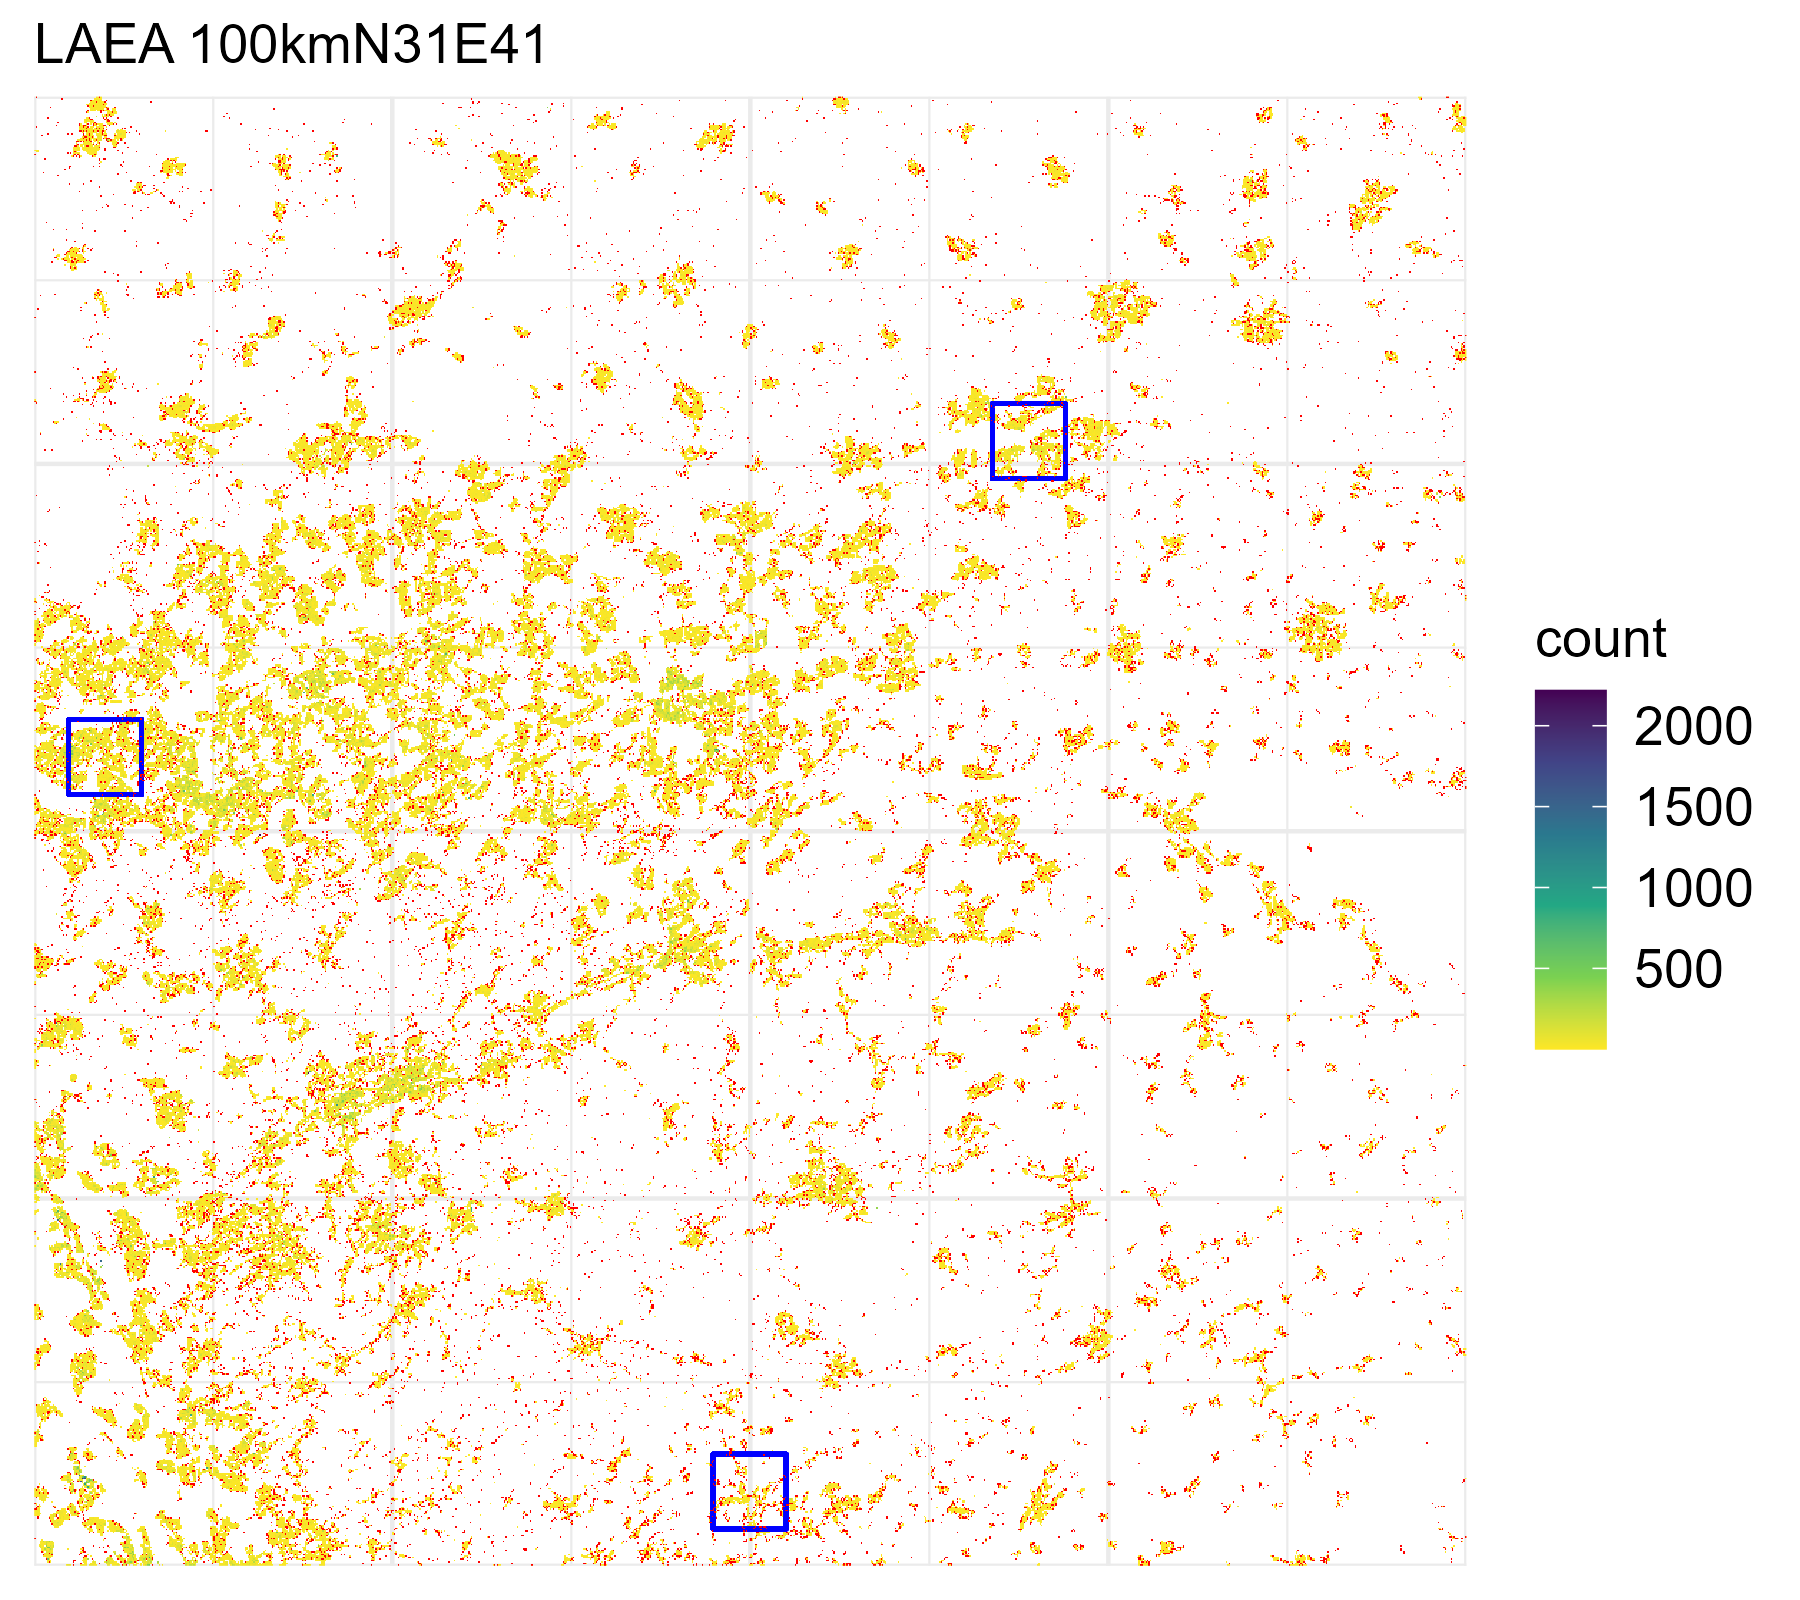
\includegraphics[width = 0.77\linewidth]{figures/CaseStudy_CKM/laea_100kmn31e41_cs.png}
    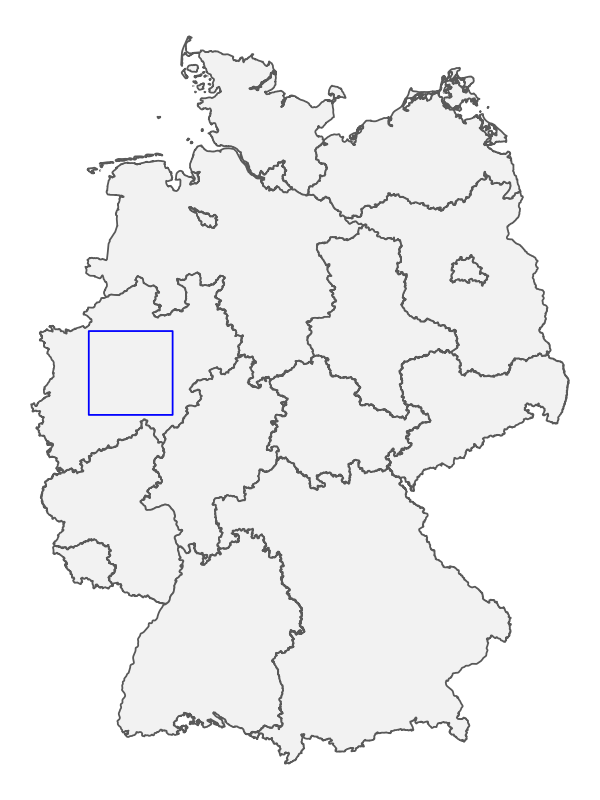
\includegraphics[width = 0.22\linewidth]{figures/CaseStudy_CKM/region_select_cs.png}
    \caption{Overview and geographic position of case study data: Inhabitants aged 50 or older by 1ha grid cell; blue frames show the position of focus areas; red pixels indicate risky cells.}
    \label{fig:cs_data}
\end{figure}

In order to examine later-on the effects of SDC also on a more local level, we furthermore define three \emph{focus areas} of 5km $\times$ 5km size (blue frames in the big map of Fig. \ref{fig:cs_data}), such as a user might wish to investigate to get information on their neighborhood.
Focus areas are selected to cover a variety of structural characteristics: area 1 (center west) is of dense urban type; area 2 (north-east) is mixed urban / suburban with medium-level population density; area 3 (south) is a low-density rural region. Close-ups are shown in Fig. \ref{fig:cs_rckm_fa} (top row).\footnote{
    Please note: In order to make the case study reproducible, we do not use actual confidential data, but create an artificial data set from published Census 2011 results which aims to replicate approximately the spatial distribution of the target population. Links to publicly available input data, as well as the steps to create the data set used in our case study can be found in the accompanying R code.}

\section{Assessing risk} \label{sec:csCKM_risk}

\subsubsection{Minimum frequency criterion}

For our application we consider a cell as sensitive if the corresponding count is smaller than 3. This corresponds to the minimum frequency criterion from section \ref{sec:risk_aggr_geosp}. In Fig. \ref{fig:cs_data} and \ref{fig:cs_rckm_fa} cells at risk are marked in red. Sensitivity measures for the full grid and the three focus areas are shown in table \ref{tab:cs_risk}. Overall, 22.5\% of inhabited cells are sensitive according to our criterion. 1.4\% of the target population is situated in these sensitive cells. The measures vary strongly between focus areas: Whereas the population in high-density area 1 is less vulnerable than the overall population, that in low-density area 3 is more vulnerable. This mirrors prior considerations from section \ref{sec:ident_geochar}.

\begin{table}[H]
    \centering
    \begin{tabular}{l c c c c}
         & full & focus area 1 & focus area 2 & focus area 3 \\
         \hline
         cells at risk (\%) & 22.5 & 9.6 & 15.0 & 34.9 \\
         pop. at risk (\%) & 1.4 & 0.4 & 0.8 & 5.7 \\
         \hline
    \end{tabular}
    \caption{Sensitivity measures for unprotected aggregates}
    \label{tab:cs_risk}
\end{table}

\subsubsection{Differencing}

144 local administrative units (LAU) overlap the study area. The same age stratification will be available for them in the census context, hence we
must assume there would be a notable risk for geographic differencing (see section \ref{sec:risk_diff}). We do not assess this risk 
here explicitly; instead we rely on the implicit protection against it provided by CKM (see \ref{sec:ckm_risk}).

\section{Applying CKM} \label{sec:csCKM_applyCKM}

We use the R package \texttt{ptable} to create the noise distribution.\footnote{
    See \url{https://cran.r-project.org/package=ptable}. The underlying method is described in \citet{Giessing2016}.}
In doing so, we want to mitigate the risk to small counts as per \ref{sec:csCKM_risk}. Therefore we set up the noise such that no 1s (or alternatively: no 1s or 2s) remain in the data. For the central CKM parameters\footnote{
    Recall from section \ref{sec:ckm_risk} that these would only be known internally to a National Statistical Institute or similar body, since we advise against publishing them together with the data.} 
we consider two sets for comparison:
\begin{itemize}
    \item variant I: max. noise = 4, noise variance = 1.8, small ct. threshold = 1
    \item variant II: max. noise  = 6 , noise variance = 2.5, small ct. threshold = 2
\end{itemize}
Remember from section \ref{sec:ckm} that the maximum noise value works in both directions, i.e. for variant I the perturbation will be between -4 and 4. The small counts threshold restricts output counts to values above the threshold (e.g. to 3 or higher for variant II).
This gives us the noise distributions shown in Fig. \ref{fig:cs_pt}.

\begin{figure}[H]
    \centering
    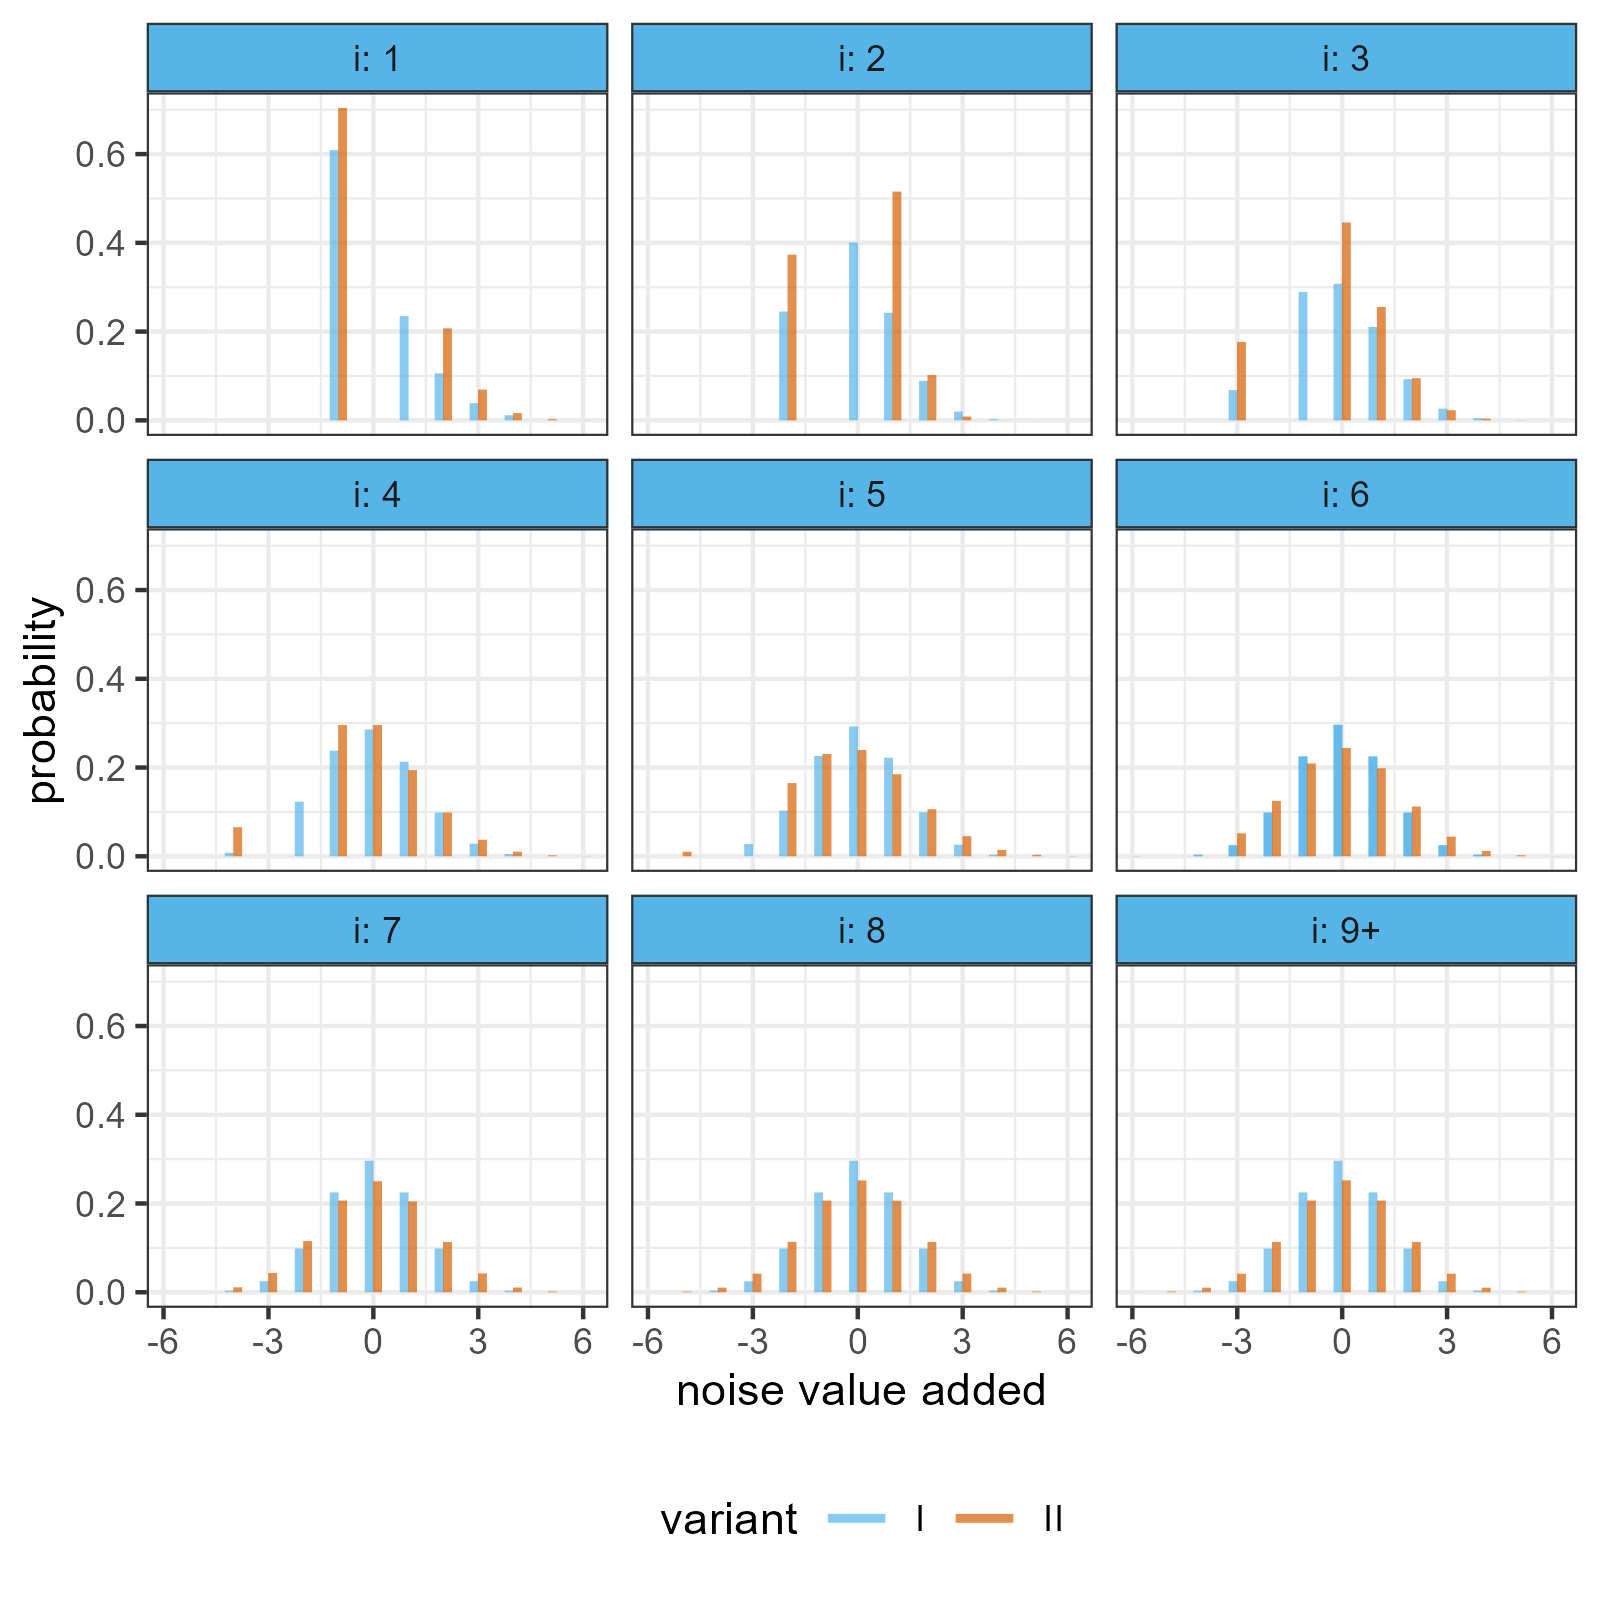
\includegraphics[width=0.9\linewidth]{figures/CaseStudy_CKM/pt_casestudy2.png}
    \caption{Distributions of the additive noise component of CKM, depending on original count $i$; all counts of 9 or above will be perturbed with the symmetric noise distribution on the bottom right; for details see \cite{Enderle2023}.}
    \label{fig:cs_pt}
\end{figure}

The figure is read as follows: If the confidential original cell count is $2$ (second graph in the top row), the probability that the added noise is $-2$ (for a perturbed count of 0) is approx. 25\% for variant I and 37\% for variant II; the probability of added noise $+1$ (for a perturbed count of 3) is approx. 24\% (variant I) or 51\% (variant II). The probability of no noise is exactly zero for variant II, since we do not allow 2s to remain in this variant. 
On the other hand, for counts 9 or higher -- depicted on the bottom right -- the probability that no noise will be added is approx. 30\% in variant I and 25\% in variant II. The probability for such counts to be changed by 5 or more in either direction is ca. 0.4\% for variant II and exactly zero for variant I (which has a maximum deviation of 4). The reason why we use different noise distributions for smaller values is mainly that we need to avoid producing negative counts.

Before creating grid aggregates we already assigned each population unit a random number between 0 and 1 (a record key) using a random number generator. When counting units for each grid cell we also aggregate these record keys as described in \ref{sec:ckm_mecha}. The resulting cell keys are used to look up for each grid cell the noise value that will be added, as shown in Fig. \ref{fig:cs_lu} (which is just Fig. \ref{fig:cs_pt}, bottom right, shown as a cumulative distribution function).\footnote{
     A note on tools: We implemented CKM here within the grid framework of the R package \texttt{sdcSpatial}, extended by a manually coded lookup step. An alternative would be modeling the grid as table (as shown in section \ref{sec:ckm}) and using the lookup step already available in the R package \texttt{cellKey}.}

\begin{figure}[H]
    \centering
    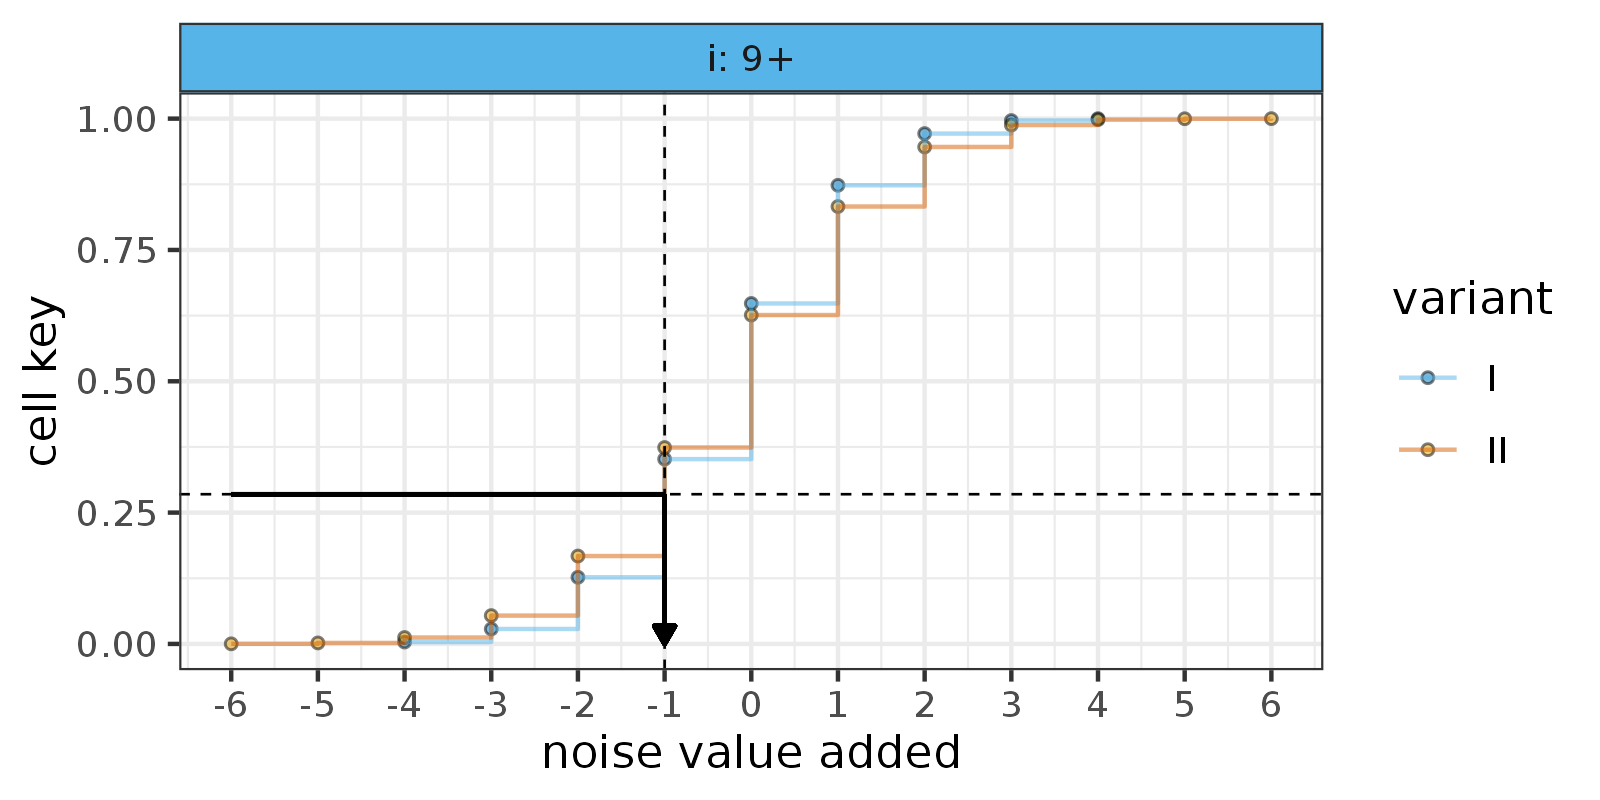
\includegraphics[width=\linewidth]{figures/CaseStudy_CKM/lookup_castestudy.png}
    \caption{Lookup step of the CKM noise mechanism: Assume for example an original count of 41 and a cell key of 0.285. We use a cumulative version of the appropriate distribution from Fig. \ref{fig:cs_pt} (here: case 9+ since $41 \geq 9$) and check in which interval the cell key falls to derive the noise value. We get $41 - 1 = 40$ as perturbed count (in both variants).}
    \label{fig:cs_lu}
\end{figure}

\section{Assessing protection results} \label{sec:csCKM_il}

\subsubsection{Visual comparison}

At first we are interested in any change the perturbation may have infused in the overall visual impression of standard choropleth maps. To this end Fig. \ref{fig:cs_rckm_fa} plots a close-up of our three focus areas -- the top row is the original (unperturbed) map of counts; the rows below are protected by CKM variants I and II. Aside from the sensitive cells (red), our chosen CKM parameters seem to preserve visual fidelity well. It is also easy to see that originally uninhabited regions (rivers, acres, etc.) remain so after SDC.

\begin{figure}[H]
    \centering
    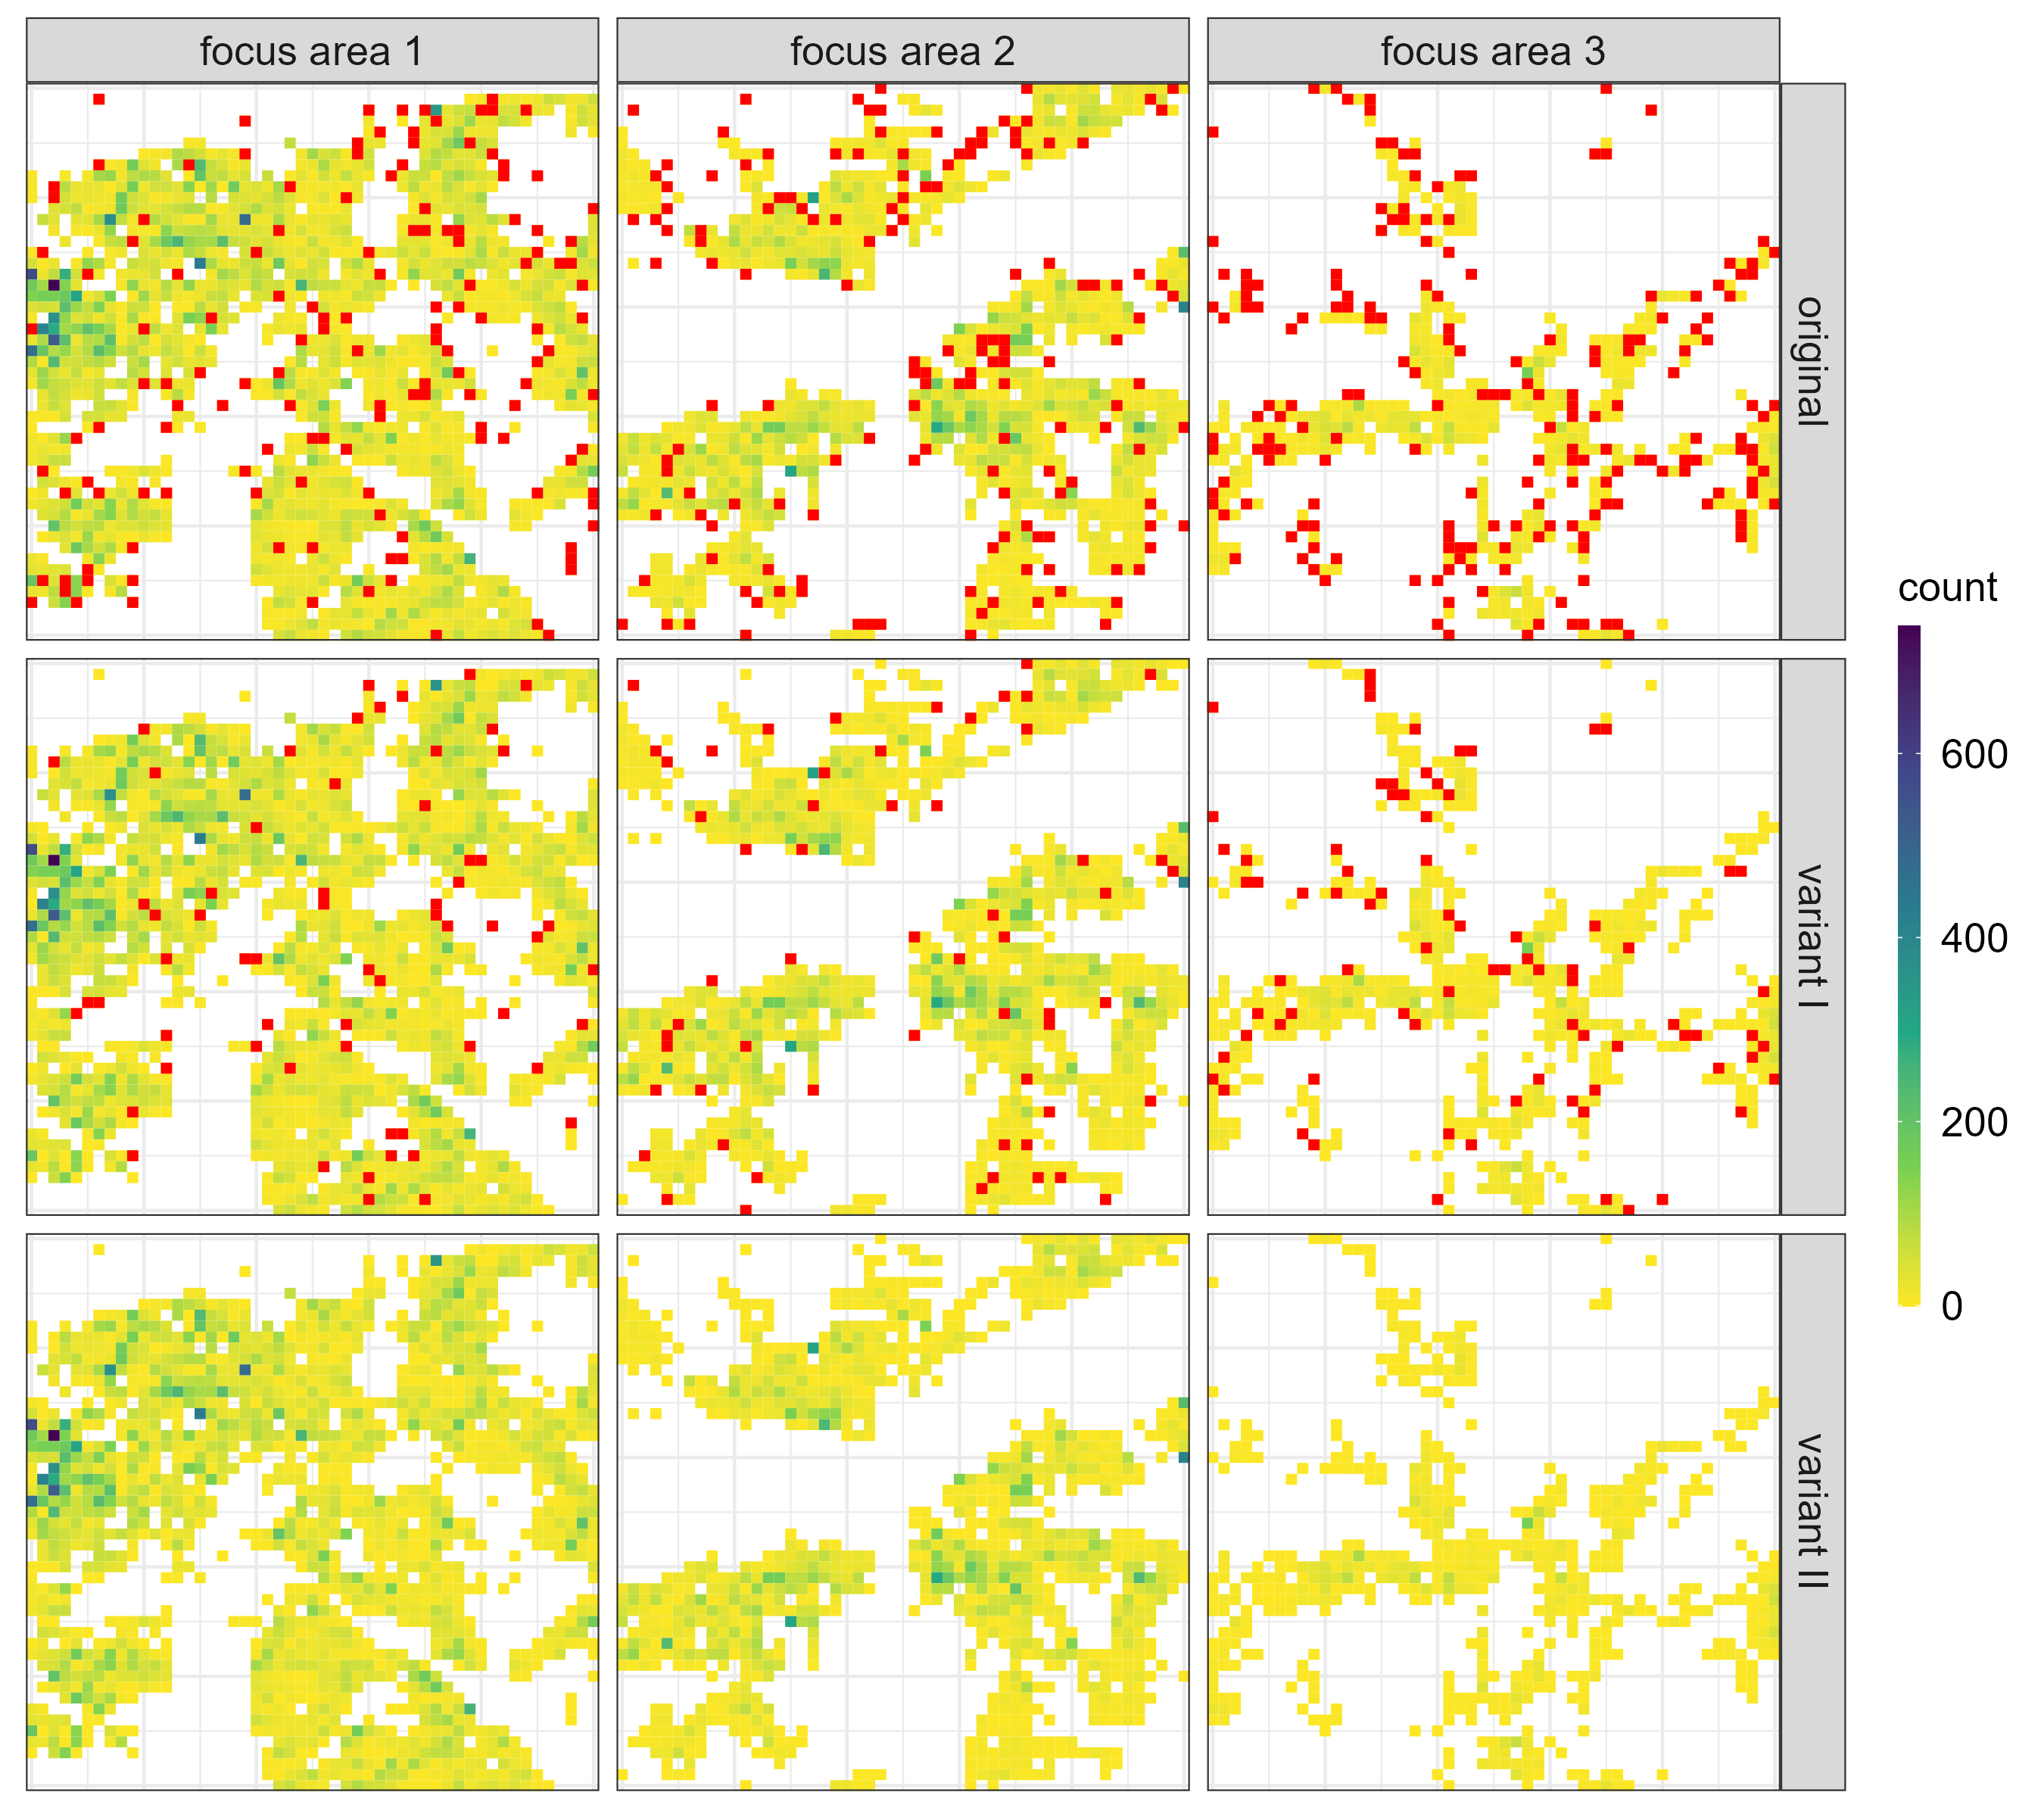
\includegraphics[width = \linewidth]{figures/CaseStudy_CKM/r_ckm_fa.png}
    \caption{Close-up of focus areas: Inhabitants aged 50 or older by 1ha grid cell; variant I and II are after CKM; red cells have counts below 3.}
    \label{fig:cs_rckm_fa}
\end{figure}

\subsubsection{Re-assessing risk after protection}

We have set up variant II of CKM such that no 1s or 2s remain in the output. 
%(by setting $j_s = 2$). 
These small counts have become either 0 or 3 or higher, according to the probability distributions depicted in the first two graphs of Fig. \ref{fig:cs_pt}. We have therefore eliminated risky small counts. For variant I, on the other hand, we allowed for 2s in the protected output.
%($j_s = 1$). 
This leaves 9.3\% of cells with counts below 3 (or 4.2\%, 5.7\%, and 15.0\% in focus areas 1, 2, and 3 respectively).
Note, however, that these need not correspond to `true' 2s anymore, as a protected 2 can result from any value between 1 and 6 (according to parameter $D$). One could argue that a potential data attacker can therefore not make use of the small count anymore, as it has become unreliable. Whether or not one feels comfortable with this argument would influence the decision between variants I and II.

\subsubsection{Measures of information loss}

Table \ref{tab:cs_il} presents a collection of information loss metrics, computed in each case for the whole data set as well as for the three selected focus areas.

\begin{table}[H]
    \centering
    \begin{tabular}{l l c c c c}
        \hline
        \multirow{2}*{measure} & \multirow{2}*{variant} & \multicolumn{4}{c}{grid} \\
        & & full & focus area 1 & focus area 2 & focus area 3\\
        \hline
        MSE
         & I  & 1.80 & 1.82 & 1.84 & 1.90 \\
         & II & 2.50 & 2.48 & 2.50 & 2.69 \\
        %\hline
        MAE
         & I  & 1.04 & 1.05 & 1.05 & 1.10 \\
         & II & 1.25 & 1.24 & 1.26 & 1.36 \\
        %\hline
        HD
         & I  & 0.067 & 0.036 & 0.056 & 0.134 \\
         & II & 0.080 & 0.043 & 0.064 & 0.162 \\
        %\hline
        KWD
         & I  & 0.119 & 0.029 & 0.061 & 0.180 \\
         & II & 0.133 & 0.033 & 0.070 & 0.219 \\
        \hline
        VMR
         & orig. & 111.50 & 94.22 & 71.18 & 26.89 \\
         & I     & 111.58 & 94.35 & 71.26 & 27.16 \\
         & II    & 111.62 & 94.41 & 71.30 & 17.24 \\
        %\hline
        MMR$^*$
         & orig. & 1.96 & 1.19 & 1.52 & 1.62 \\
         & I     & 1.68 & 1.06 & 1.34 & 1.04 \\
         & II    & 1.63 & 1.01 & 1.24 & 1.17 \\
        %\hline
        Moran's $\mathcal{I}$
         & orig. & 0.374 & 0.321 & 0.323 & 0.298 \\
         & I     & 0.373 & 0.320 & 0.323 & 0.296 \\
         & II    & 0.373 & 0.320 & 0.323 & 0.296 \\
        %\hline
        ILM
         & I  & -0.02\% & -0.04\% & -0.03\% & -0.10\% \\
         & II & -0.02\% & -0.05\% & -0.01\% & -0.08\% \\
        \hline
    \end{tabular}
    \caption{Information loss measures for two CKM variants, applied to the full grid ($1000 \times 1000$) and three focus areas ($50 \times 50$); MSE, MAE, HD, KWD as per section \ref{sec:util_DD}, VMR, MMR$^*$, Moran's $\mathcal{I}$, ILM as per section \ref{sec:util_SPAT}; HD is rescaled to $[0,1]$; KWD is exact for focus areas and approximated with approximation parameter $L = 3$ for the full map, using an additive measurement error to deal with mass gaps \citep{RicciatoGualandi2024}; for details see accompanying R code.}
    \label{tab:cs_il}
\end{table}

The upper part contains measures of distributional distance: mean squared error, mean absolute error, Hellinger's distance, and Kantorovich-Wasserstein distance. Most of them are useful for comparison between the two variants, but do not have an intuitive interpretation. The MAE is an exception: Since CKM applies to each (inhabited) grid cell, this metric gives us the approximate expected error in the count value of any given cell. We see that it is independent of the scope of a map and comes to ca. 1.0--1.1 for variant I and ca. 1.2--1.3 for variant II. HD and KWD are both relatively close to zero, which implies that the distribution is generally well preserved. We observe a somewhat higher information loss in the rural focus area 3 than in the urban areas 1 and 2. This is in line with expectations: Counts of only 1, which are never preserved, occur more frequently in sparsely populated areas, and the same error level in absolute terms has a stronger relative effect, if counts are small and sparse.

The lower part of table \ref{tab:cs_il} shows measures of spatial association: Variance-mean ratio, MedAD-median ratio, Moran's $\mathcal{I}$, and information loss measure based on Moran's $\mathcal{I}$. Comparing for the first three the value of original data with CKM variants I and II we see overall little change (slightly more for MMR$^*$), implying that spatial characteristics of the areas in question remain intact. The ILM measure correspondingly is almost zero, showing very little loss of spatial information.

\subsubsection{Local information loss}

Fig. \ref{fig:cs_ilcell_ilmw} (top) shows the absolute error per cell resulting from CKM (see table \ref{tab:util_cellLVL} in section \ref{sec:util_LOC_cellerror}), while Fig. \ref{fig:cs_ilcell_ilmw} (bottom) is the smoothed version using the moving window method from section \ref{sec:util_LOC_mw}. Note that the absolute error per cell is limited by 6 for CKM variant II and 4 for CKM variant I, as per parameter $D$. Moreover, the error distribution is not spatially correlated, meaning it should average out well when looking over a given map section. This can be seen directly in Fig. \ref{fig:cs_ilcell_ilmw} (bottom), where the maximum error could be as high as 4 or 6 respectively, but no such dark spot occurs. In fact, the highest mean absolute error (MAE) of a focal region is 1.64 for variant I or 1.96 for variant II. In other words, for any arbitrary section of 5 $\times$ 5 grid cells (500m $\times$ 500m) a user could be interested in, the average deviation in counts can be guaranteed to be below 2.

Finally, Fig. \ref{fig:cs_locI} displays estimates for the local (cell-level) Moran's $\mathcal{I}$ statistic from section \ref{sec:util_moran}. A strong resemblance between original and perturbed versions implies that for both CKM variants the structure of spatial autocorrelation is well preserved.

\section{Concluding thoughts}

We intended this case study to be merely illustrative for the metrics and concepts introduced before. In practical application, several further steps would need to follow, including, but not limited to:
\begin{itemize}
    \item comparing CKM with other SDC methods (see chapter \ref{sec:methods}),
    \item further tweaking CKM parameters to reach the best trade-off between risk mitigation and accuracy; see also \citet[~ch.4]{Guidelines3_CensusDemog},
    \item repeating the analysis for other demographic breakdowns and potentially a more diverse set of focus areas,
    \item communicating the findings to prospective users and collecting feedback,
    \item addressing non-statistical challenges, like implementation of the method in production systems and processes, or issues of user communication \citep[~ch.5]{Guidelines3_CensusDemog}.
\end{itemize}

\begin{figure}[H]
    \centering
    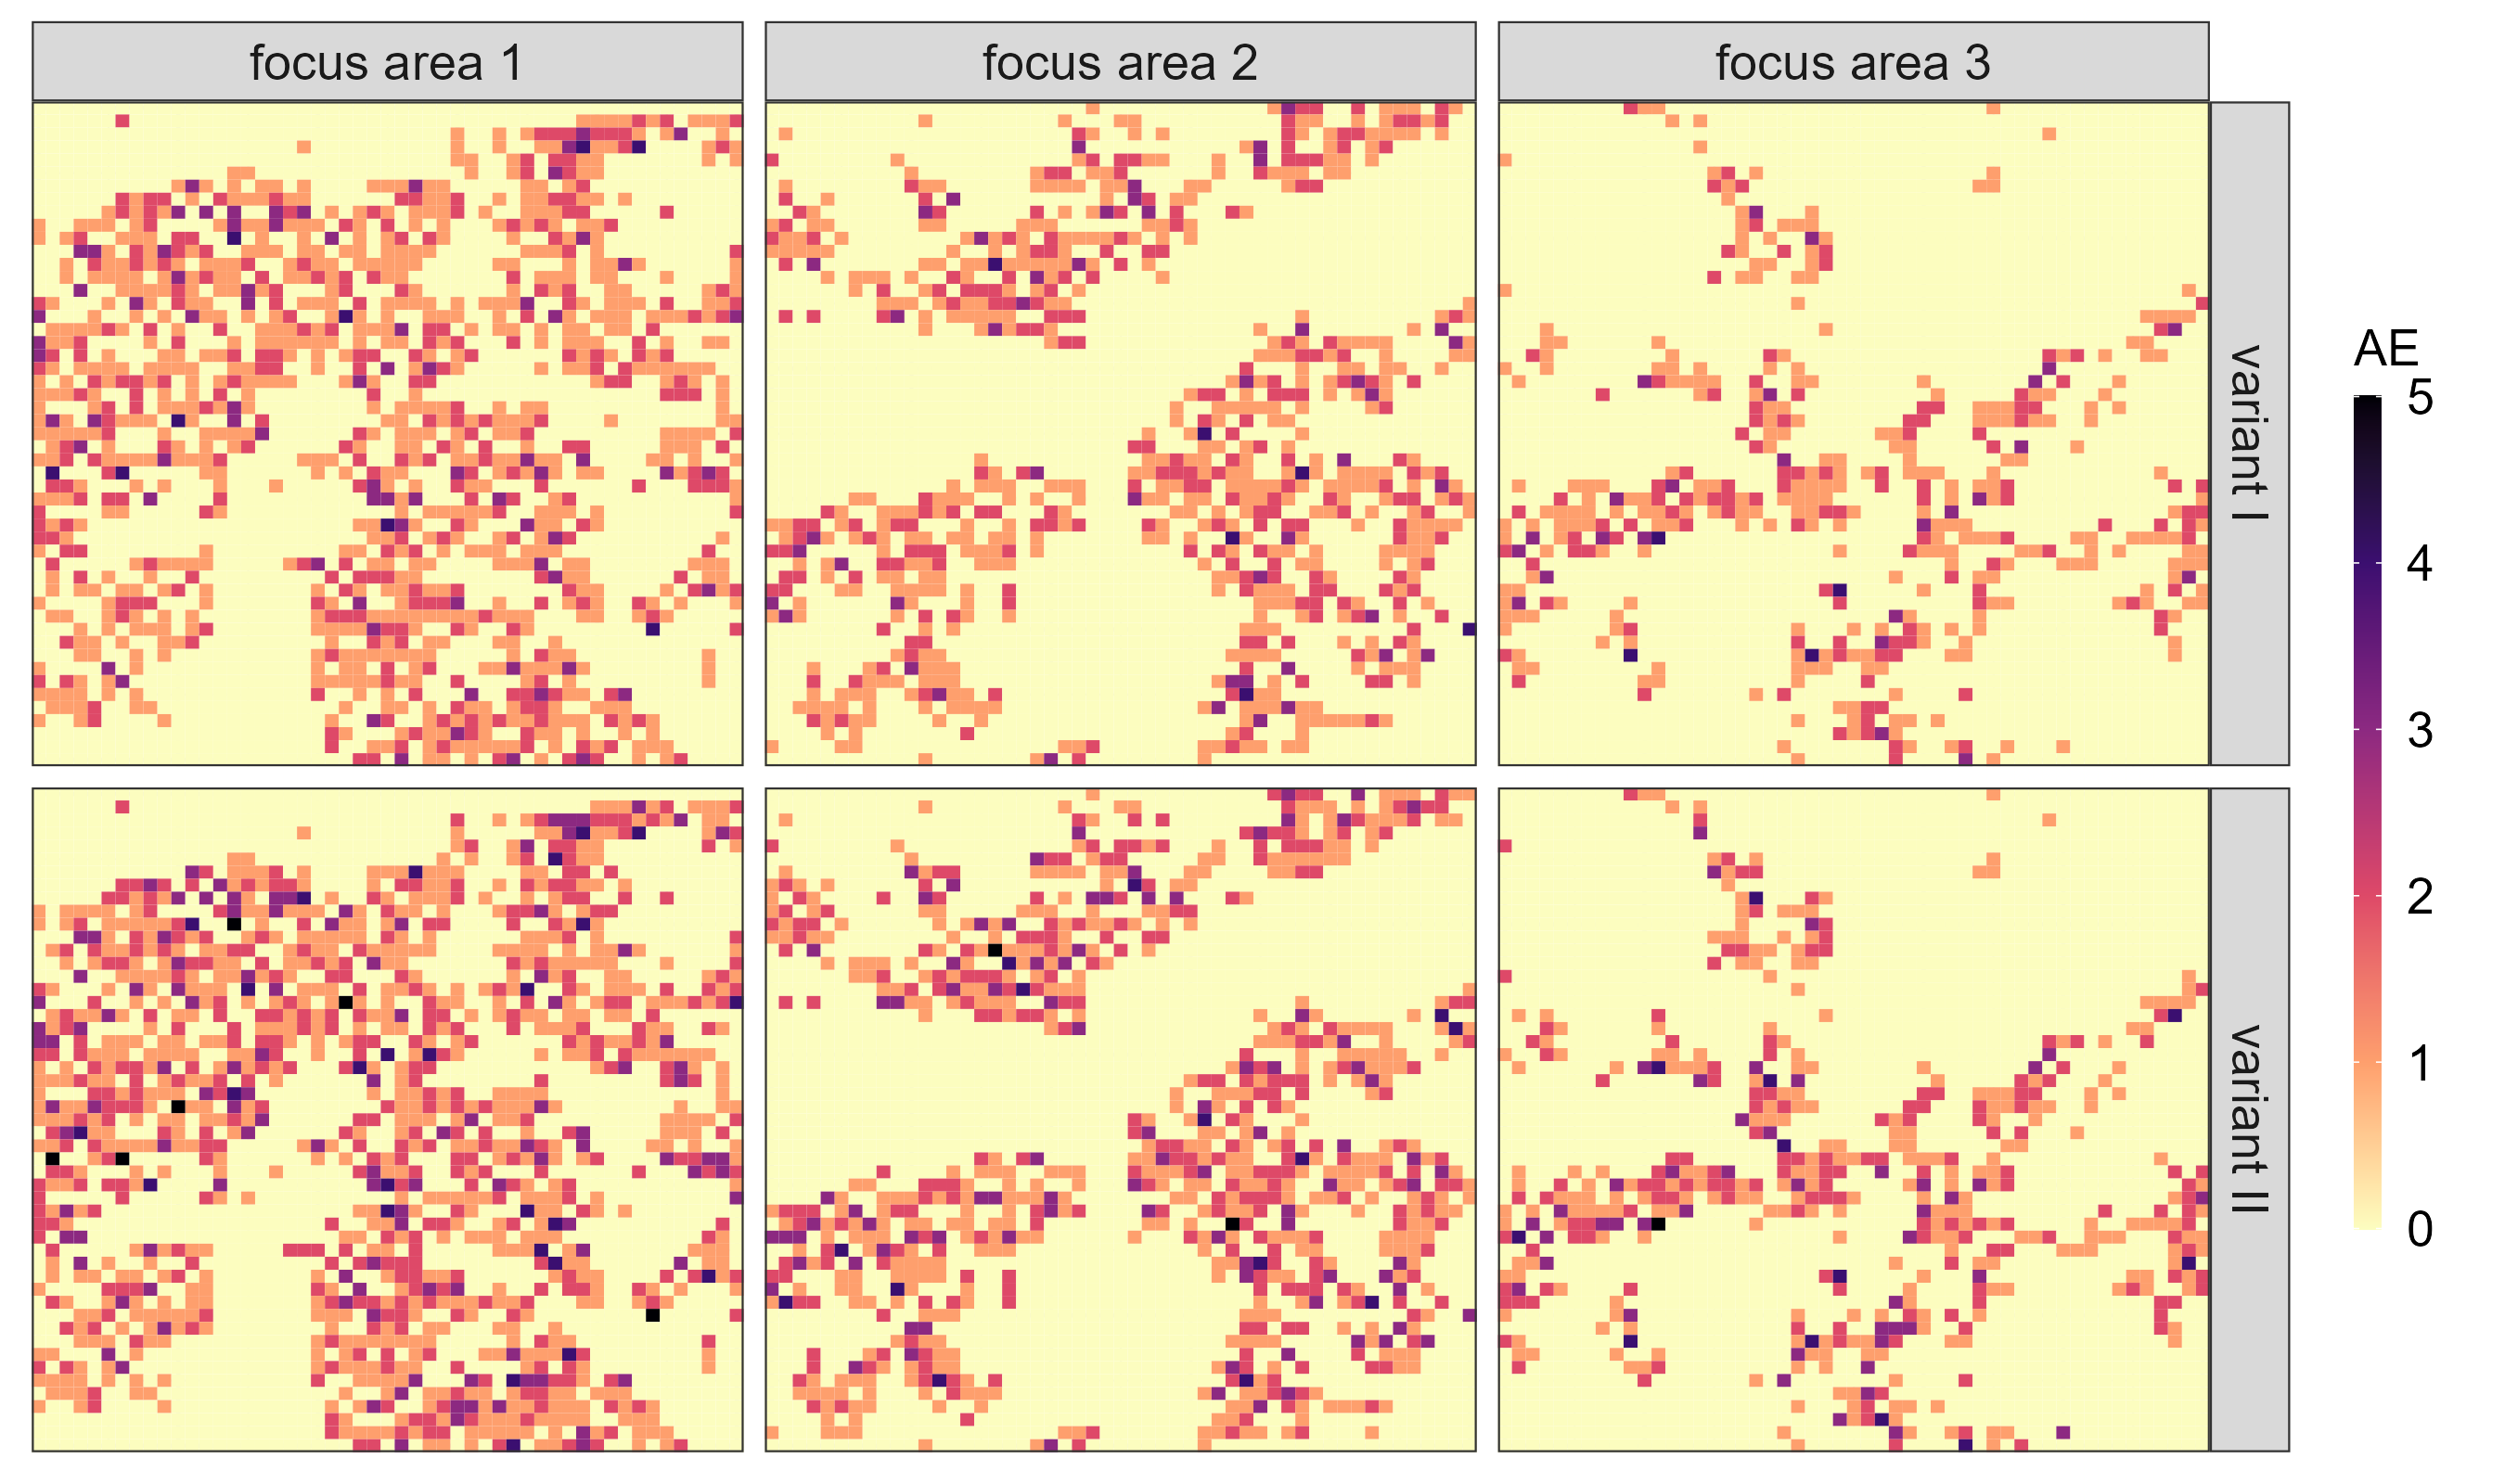
\includegraphics[width = \linewidth]{figures/CaseStudy_CKM/r_ilcell.png}
    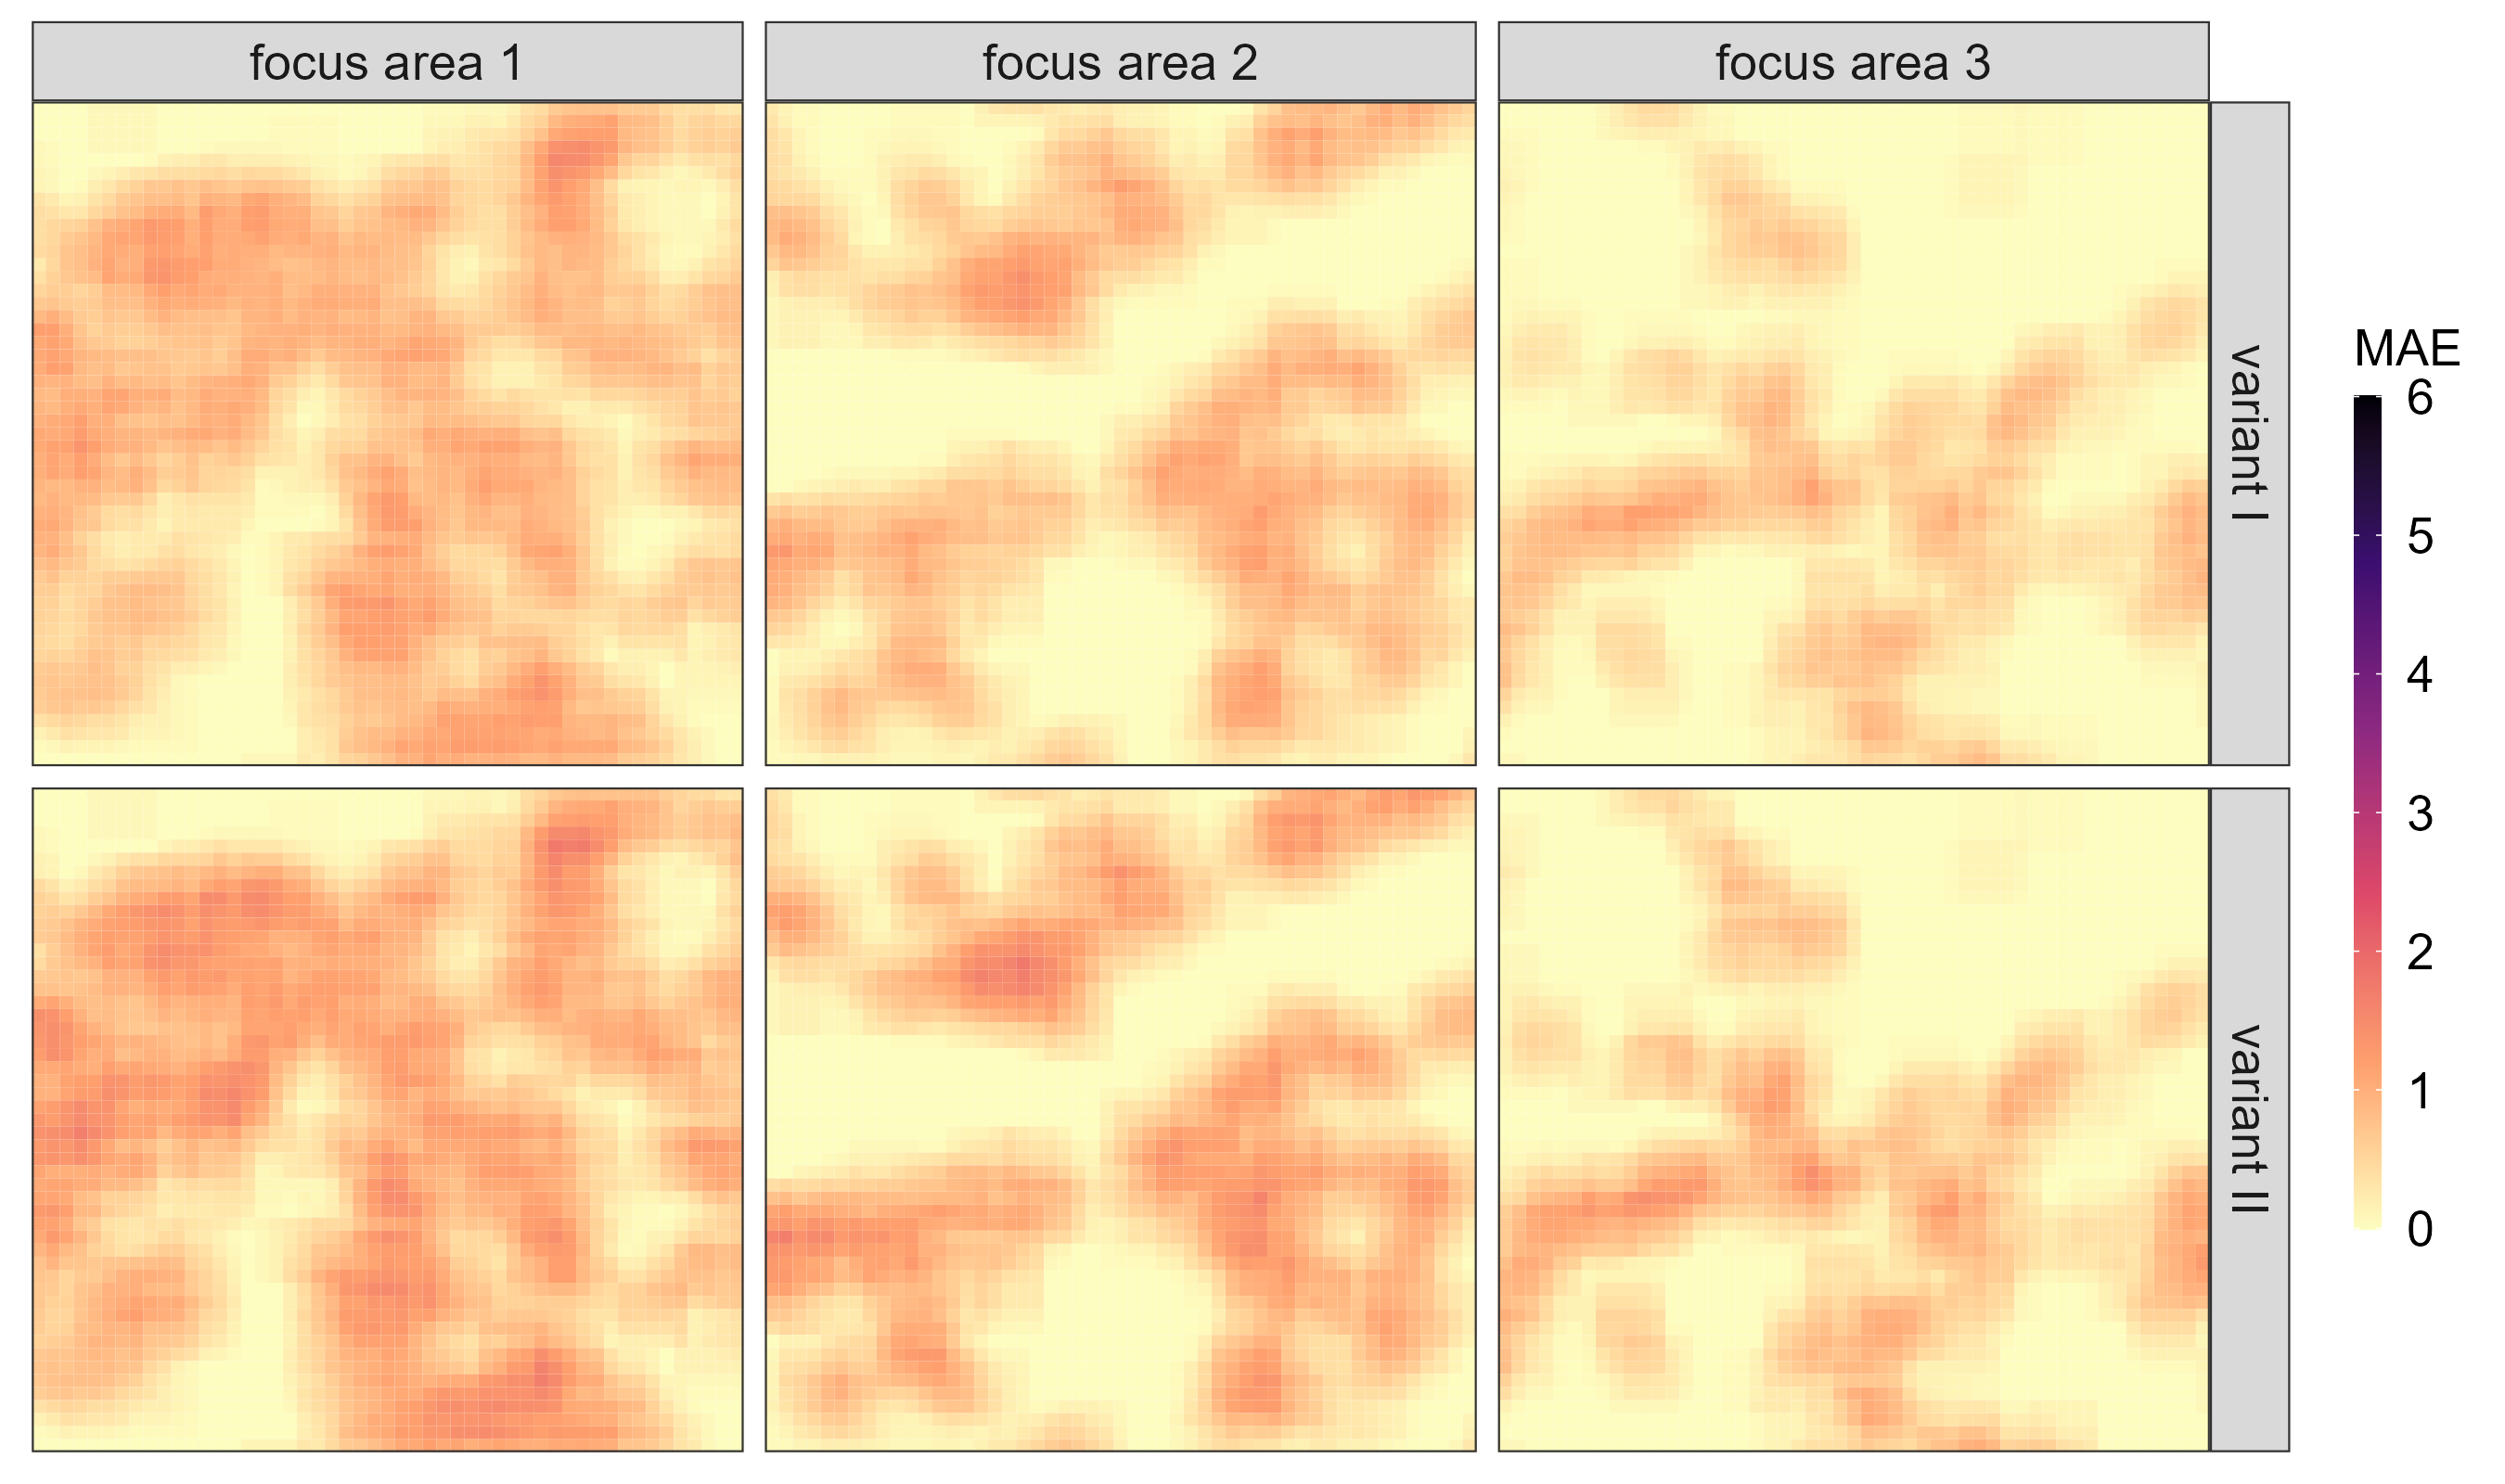
\includegraphics[width = \linewidth]{figures/CaseStudy_CKM/r_il_mw.png}
    \caption{Top: Maps of cell-level absolute error (AE); bottom: smoothed error maps, using the moving window approach with mean absolute error (MAE) measure and a $5 \times 5$ moving window.}
    \label{fig:cs_ilcell_ilmw}
\end{figure}

\begin{figure}[H]
    \centering
    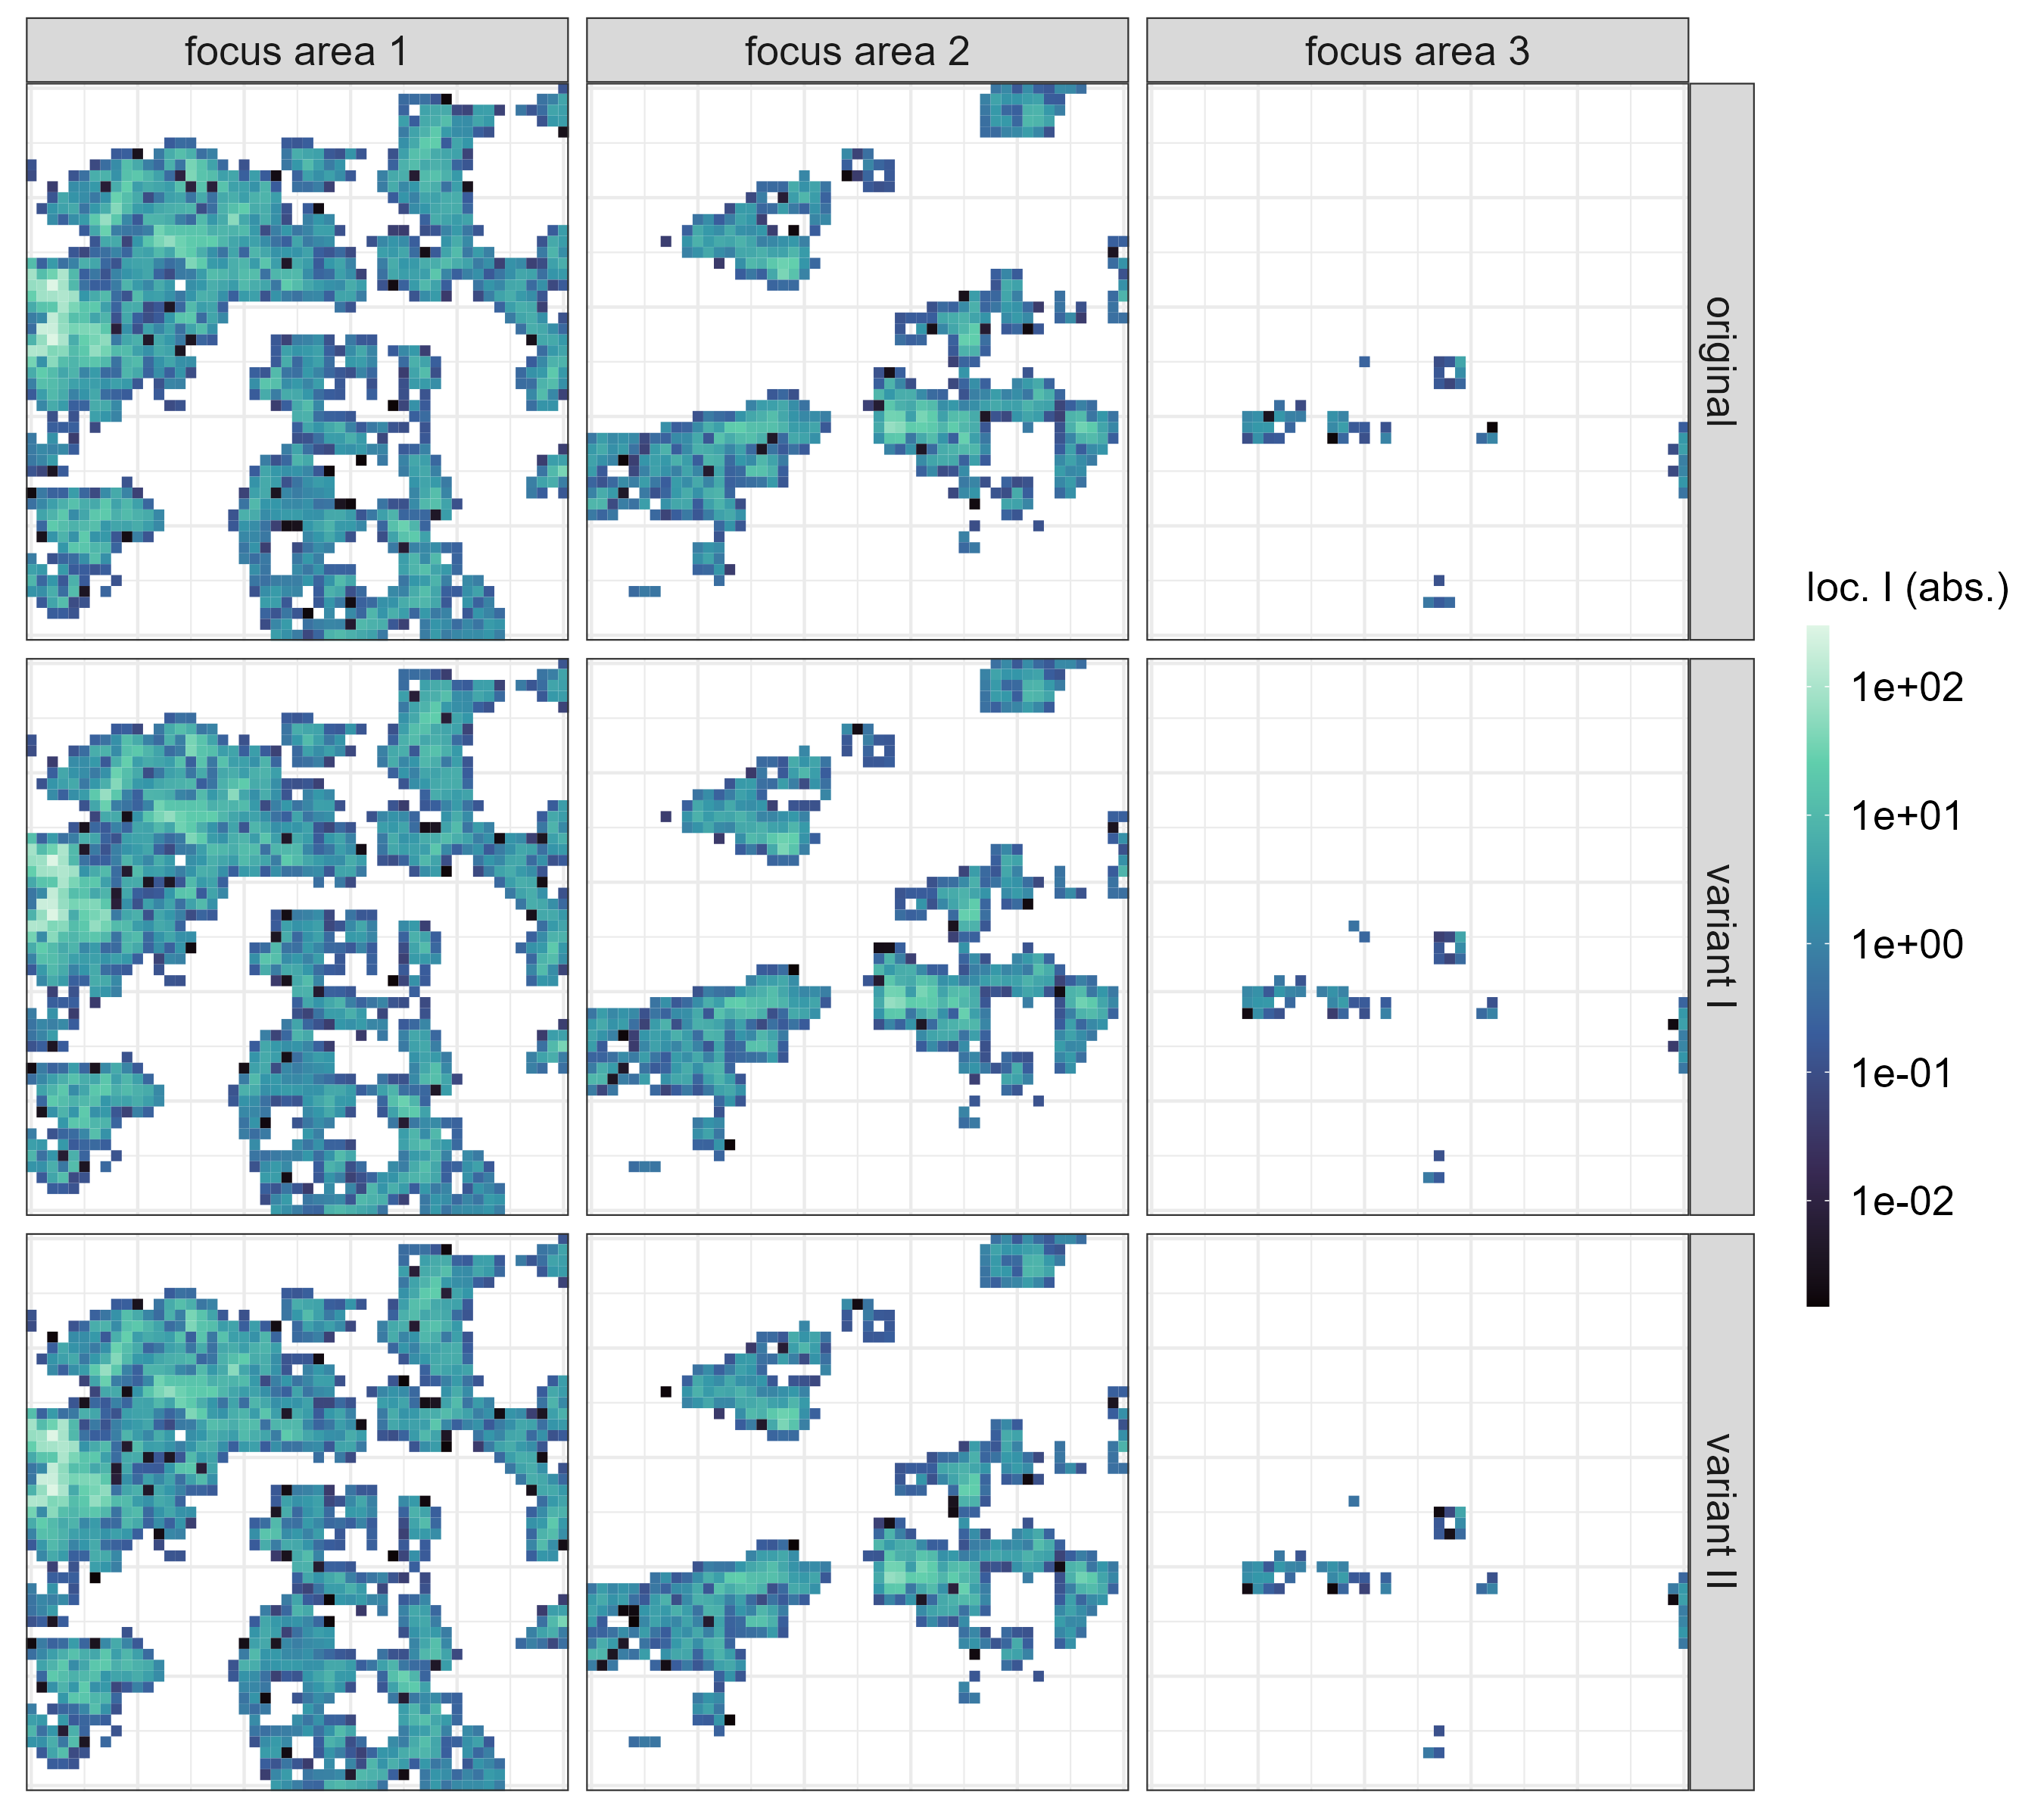
\includegraphics[width = \linewidth]{figures/CaseStudy_CKM/r_locI_fa.png}
    \caption{Maps of local Moran's $\mathcal{I}$ (absolute value); shown are only grid cells for which the statistic is significantly different from zero at $p \leq 0.05$.}
    \label{fig:cs_locI}
\end{figure}

